\section{Related Work}
\label{sec:related}
%\emph{\color{red}Related work including a short section of foundational work in the area of your thesis, a section on directly relevant work and how your proposed work either leverages that work (e.g., techniques you plan to adopt) or differs from it (e.g., novel contributions), and a description of how your proposed work is distinct from the work being done by your colleagues at UW.}

The work related to this thesis proposal falls broadly into three categories: architectures for wireless networks, mechanisms to optimize configuration of a single wireless link, and mechanisms to optimize configuration for concurrent workloads.

\subsection{Background on Wireless Network Architectures}
There are three major architectures used in Wi-Fi networks today. We begin with an in-depth discussion on access point networks, and then summarize wireless mesh networks and the new Wi-Fi Direct specification for peer-to-peer wireless networks.

\subsubsection{Access point networks} The first type, and the one most commonly used in the home, is an \emph{access point network}~\cite{80211,nagus_homerf} (\figref{fig:ap_network}). The network is organized in a star topology, with the AP at the root and all clients operating on the same channel. The AP has a (typically wired) uplink connection to the Internet gateway, such as a DSL, FiOS, WiMAX, or cable modem. Topologically, the access point model provides a simple abstraction: it ignores the broadcast nature of wireless networks, and instead acts as an Ethernet switch (for the wireless LAN) and either an Ethernet bridge or IP router (for the uplink). The AP (or the network behind it) represents a central point for admission control, including IP configuration via DHCP, and DNS and NAT services. As if all the connections were wired, all transmissions from clients are sent to the AP, which routes these transmissions as appropriate, either back onto the wireless LAN for wireless clients, and otherwise out of the uplink connection. The primary constraint imposed by wireless is that, network wide, there can only be one ongoing transmission at a time. This is enforced by a simple CSMA/CA~\cite{karn_maca} mechanism and the optional use of RTS/CTS when there exist hidden terminals in the network.

\heading{Power save mode.}
In 802.11, access points also include specialized functionality that allows clients to conserve energy by putting their RF hardware to sleep. The AP buffers downlink packets for sleeping clients, which poll the AP for new traffic when they wake. When any client is asleep, the AP also buffers multicast and broadcast traffic, offloading these periodically every few beacons, typically with a period 200\ms--400\ms. However, the standard Wi-Fi contract mandates that the AP never sleeps---clients can contact the AP to send data or poll for traffic at any time.

\heading{Network extenders.}
Note that in large homes, the access point may have insufficient range. Thus the standard generalizes the star topology slightly to allow for wireless repeaters that act as Ethernet bridges to extend the AP network. These repeaters operate on the same channel as the AP and broadcast the same BSSID\@. They also offer the same contract as APs: they perform buffering for sleeping clients, and are not allowed to sleep themselves.

\heading{Wireless distribution system.}
Finally, in some cases there can be multiple access points that are connected via a wireless backbone. This is commonly the case in enterprise environments, in which APs are deployed as gateways for mobile to the larger wired LAN\@. In the home, some companies now offer ``dual band'' APs that include two NICs and act as two logical APs using the same SSID, one each on the 2.4\GHz and 5\GHz frequency bands. Dual band functionality maintains support for cheap devices that only operate on 2.4\GHz---which is often plagued by interference from microwaves, Bluetooth, and neighboring LANs---while allowing highly capable devices to use the 5\GHz frequency band which includes 24 non-interfering channels and provides better isolation from neighboring networks. In both these cases, the wireless access point networks operate as described above, independently and without cross-AP coordination, and only communicate via the wired backplane.

\heading{Network discovery.}
To join a wireless network, a client first conducts a scan by hopping through the available 802.11 channels and sending on each a link-layer broadcast packet called a Probe Request. Devices that offer network functionality, i.e.\ APs or extenders, respond to these probe requests with information about the network (SSID, AP MAC address, type of security, etc.) and a list of their capabilities (e.g., the bandwidth of the channel and the number of MIMO streams that the AP supports). A client selects between responding devices via local policy, but in practice clients simply select the AP with the strongest measured signal strength, or preferentially select the 5\GHz network when it meets a minimum signal strength threshold.

\heading{Summary.} Access point networks provide a simple wireless switch abstraction that works well, and this has driven the dramatic growth of Wi-Fi that continues today. However, as applications in the wireless home become more demanding, AP networks will be limited by their inability to support more efficient communication patterns when possible and their spectrally inefficient use of only one channel. We believe that a more flexible network is needed to enable these applications.

\begin{figure}[thp]
      \centering
      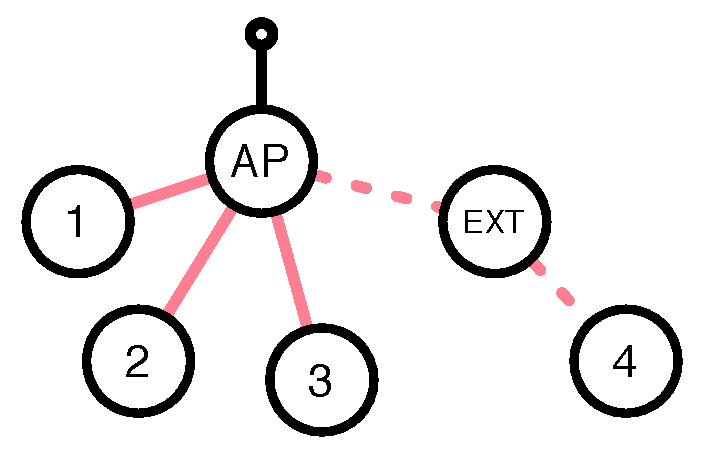
\includegraphics[width=0.8\columnwidth]{figures/omni/ap.pdf}
      \caption{\label{fig:ap_network} An access point network is structured as a star topology in which all nodes communicate on the same channel and talk directly to the access point. Optionally, wireless extenders can act as repeaters for distant clients (dashed lines) on the same channel.}
\end{figure}
\begin{figure}[thp]
      \centering
      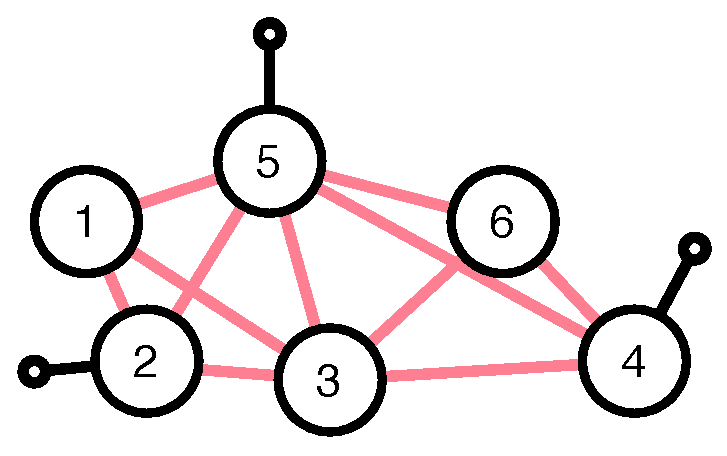
\includegraphics[width=0.8\columnwidth]{figures/omni/mesh.pdf}
      \caption{\label{fig:mesh} An mesh network is an unstructured topology in which any nodes on the same channel can communicate. There may be multiple egress points to external networks. In most work, the mesh uses a single channel, though in some cases (not pictured), nodes with two or more radios can use multiple channels.}
\end{figure}
\begin{figure}[thp]
      \centering
      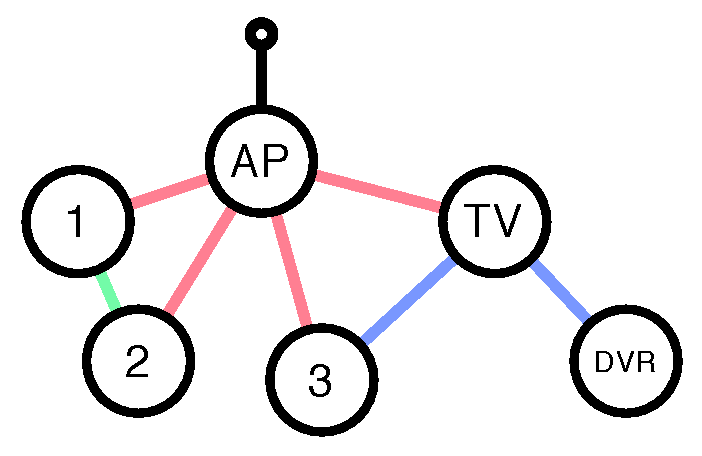
\includegraphics[width=0.8\columnwidth]{figures/omni/p2p.pdf}
      \caption{\label{fig:wifi_p2p} A Wi-Fi Direct ``peer-to-peer'' network enables devices to concurrently act as clients in one access point-like network while serving as members of another. Thus device-to-device communications, e.g., between nodes 1 and 2 or between the TV and DVR can happen directly and on different channels, hence different contention domains, than other ongoing communications.}
\end{figure}
\subsubsection{Mesh networks}
The second type of wireless network is a mesh network (\figref{fig:mesh}). In a mesh, the nodes are spread over a much larger area and offer Internet service to clients that are typically separated from gateways by several hops~\cite{whitehead_mesh}. Two instance of this include Rice University's TFA project~\cite{camp_tfa,rice_tfa}, which provides Internet connectivity to low income urban neighborhoods in Houston, and Meraki~\cite{meraki}, which provides wireless coverage for hotels. There are also research mesh networks, such as Roofnet~\cite{bicket_roofnet}, which study the generalized problem of routing traffic in many directions across a mesh without a specific application.

The main problems in mesh networks are caused by their large spread and resulting many-hop paths. For instance, much of the research on mesh networks focuses on maintaining a distributed routing infrastructure~\cite{stuff}, pipelining transfers along long mesh paths~\cite{li_blockswitched,li_mesh,rodrig_thesis}, using network coding to improve performance of crossing flows~\cite{katti_xors,katti_anc}, or propagating data more effectively across the network by making use of many unreliable links~\cite{biswas_exor}. As a result of the complex nature of these solutions, work on mesh networks tends to simplify other aspects of network design, for instance by using homogenous single-antenna nodes, or fixing the entire network to a single bitrate.

\heading{Summary.} In our view, mesh networks are poorly matched to the home. The hard problems in mesh revolve around the sparsity of nodes, low quality of links, and long paths. In contrast, the constrained spacing and dense deployment of devices will make paths in the home likely to be short---at most a few hops---and of high bandwidth, which should be manageable by simpler mechanisms. Instead, the problems that mesh work ignores, such as heterogeneous devices and rate adaptation, are likely to be the hard problems in the home.
 
\subsubsection{Wi-Fi Direct: peer-to-peer networks}
The third type of wireless network is a Wi-Fi Direct ``peer-to-peer'' network~\cite{wifi_direct} (\figref{fig:wifi_p2p}), which represents a middle ground between the logically centralized access point networks and the logically distributed mesh networks. The groundwork for these networks was laid by Chandra, et al.\ in MultiNet~\cite{chandra_multinet}, which enabled a client to connect to multiple APs concurrently. MultiNet virtualizes a single wireless device across multiple access points, keeping one virtual client active at a time. Inactive virtual clients in MultiNet enable power save to force APs to buffer their traffic, and in this manner, all virtual clients can maintain associativity to their respective APs. When the hardware permits fast frequency switching, MultiNet clients can even associate to APs on different channels. In the original implementation of MultiNet, only one virtual client could be active at a time, even when two operated on the same channel, because the hardware could only be programmed to associate to a single AP at a time.

In essence, Wi-Fi Direct offers a standardized, updated MultiNet interface with better device support. In particular, some NICs can be programmed with multiple BSSIDs in order to operate virtual devices on the same channel concurrently. Second, hardware manufacturers have made fast channel switching a priority, with some NICs able to switch between channels on different bands within 2\ms~\cite{atheros_ar9390}. Finally, Wi-Fi Direct better handles the case where one NIC acts as a virtual client in one network and the access point for another. If these operate on different channels, the virtual access point will have to sleep while the virtual client is active, thereby violating the standard Wi-Fi contract that access points are always available. Thus Wi-Fi Direct adds mechanisms for a virtual AP to notify clients of its absence.

\heading{Summary.} We believe that Wi-Fi Direct supports many of the protocol mechanisms we would need to build a flexible home network. For instance, it should be possible to use multiple virtual devices to build a single logically-connected network that looks like an extended access point network, but makes uses of multiple channels to separate independent device-to-device workloads. We also believe it is possible to extend these mechanisms to support short-circuited paths in the network. However, as with rate selection in 802.11n, \emph{Wi-Fi Direct provides no instruction as to how to make decisions} about when to initiate the use of multiple channels; what devices, which links, and what operating channels to choose; or how to manage the network in a distributed manner. These are among the challenges we propose to tackle in this work.

\subsubsection{Cellular networks}
Finally, cellular data networks, in particular 4G networks based on WiMAX~\cite{wimax} or LTE/LTE-Advanced~\cite{lte}, offer wireless data service over a wide (metropolitan scale) area. These networks are highly centralized, and include scheduling mechanisms to tightly control and optimize the timing, frequency use, and rate of all transmissions in the network. The purpose of a WiMAX network is not for device-to-device communication, but rather device-to-Internet. In general, the cellular data networks do not provide a suitable model to replicate in the home.

\subsection{Configuring a Single Link}
An important first step towards operating a wireless network efficiently is operating an individual wireless link efficiently. The most basic challenge is rate adaptation, the task of selecting the best transmit modulation, coding rate, antennas, and number of spatial streams that fits the underlying RF channel. There are other important single link configuration problems---such as selecting the best frequency for the link, or trying to minimize the power consumption of one endpoint---but rate selection is the studied problem in this area since a good scheme has a large effect on throughput.

In theory, it is simple to select the physical layer configuration because this is directly determined by the specifics of the RF channel. The signal-to-noise ratio (SNR) is the gold standard for performance in narrowband channels. Textbook formulas relate the error rate of different modulations to the SNR~\cite{Tse}. The best rate, channel, or transmit power is then simple to compute.

In practice, 802.11 LANs have never used channel measurements as more than a coarse indicator of expected performance. There have simply been too many ways in which the observed measurements and actual performance fail to match the predictions of theory. For example, the most accessible channel measurement is received signal strength indication (RSSI), which serves as a proxy for the true SNR\@. RSSI measurements are samples that may vary over packet reception, be mis-calibrated, or be corrupted by interference, all of which are known to be issues in practice~\cite{camp_mobicom08, judd_rate_adapt, reis_sigcomm06}. Even if RSSI were perfect, it does not reflect the frequency-selective fading of 802.11 channels, which are not close to narrowband. Nor does it account for imperfect receivers that may greatly degrade performance~\cite{aguayo_roofnet,judd_rate_adapt}. Due to these factors, the minimum RSSI at which a rate starts to work varies by more than 10\dB for real links~\cite{reis_sigcomm06, snr_infocom08, zhao_sensys03}.

Instead, a form of guided search is widely used in practice to select operating points. Packet delivery is simply tested for a rate or transmit power to see how well it works. If the loss rate is too high, a lower rate is used, otherwise a higher rate is tested. Lucent's ARF algorithm~\cite{lucent_arf}, OAR~\cite{sadeghi_oar}, and SampleRate~\cite{Bicket_SampleRate} were early rate adaptation algorithms of this type. The state of the art today is the Linux kernel's Minstrel~\cite{minstrel}, a version of SampleRate adapted for modern Wi-Fi hardware that can use lower rates for packet retransmissions. Minstrel has also been adapted for 802.11n, performing parallel searches between the multiple MIMO modes with different numbers of spatial streams and channel bandwidths. The guided search approach is very effective for slowly varying channels and simple configurations (e.g., a few rates with fixed transmit power and channel) since the best setting will soon be found.

For rapidly varying channels, these algorithms become less effective. Camp, et al.~\cite{camp_mobicom08} demonstrated the importance of varying the time constants used to generate summary statistics for Minstrel-like algorithms. Recently, RapidSample~\cite{ravindranath_sensorhints} used hints from smartphone sensors to detect mobility and switch to a simplified SampleRate-like algorithm that walks up and down the rates in an agile manner. This provides better performance when devices are moving, but it is not obvious how to extend RapidSample's logic to 802.11n where there is not a single linear set of rates.

%However, search becomes less effective as channels change more quickly and the configuration space becomes more complex. Both of these factors are trends: 802.11 clients are increasingly used when they are truly mobile, both walking and in vehicles; and NICs that are now being deployed with 802.11n depend on multiple antennas, which adds another dimension to and increases the size of the search space. Also, tuning combinations such as rate and power is much more complex. 

Recent work has returned to the theoretical approach and made headway by measuring symbol-level details of packet reception. In particular, SoftRate uses the output of soft-Viterbi decoding for each symbol to estimate the bit error rate (BER)~\cite{Vutukuru_SoftRate}. This allows it to predict the effects on packet delivery of changing the rate. AccuRate uses symbol error vectors for the same purpose~\cite{accurate_nsdi10}.  However, these methods are not defined for selecting other useful parameters, such as transmit power, and they do not extend from 802.11a/g to 802.11n, e.g., when selecting antennas or numbers of spatial streams.

\heading{Summary.}
%In theory, RF channel measurements should enable the endpoints of a link to determine useful parameters such as rate, MIMO mode, antennas, operating channel, and transmit power levels. However, the RF measurements available from commodity Wi-Fi cards are inadequate for good performance in practice. Instead, Wi-Fi uses guided search algorithms in practice, but these can complex and inefficient in rapidly varying channels. Recent work at the physical layer has moved back towards theoretical algorithms, but these are not available in hardware today and may not extend to 802.11n.
In a wireless home with competing workloads and fluctuating topology, the configuration of a single link is a small sub-problem, yet important to solve accurately and rapidly to ease the burden of higher-layer decisions. Today's algorithms are effective for static links, but likely insufficient when devices are mobile or for tasks such as selecting the best intermediary or best operating channel. As part of our thesis, we provide a better solution that works on commodity 802.11n NICs available today (\secref{sec:preliminary}).

\subsection{Managing Multiple Links}

\subsubsection{Reducing single-channel anomalies}
Rate anomaly problem~\cite{heusse_anomaly}. 802.11e batching~\cite{80211,80211n}. Multihop~\cite{rodrig_thesis,bahl_repeater}. Collisions~\cite{tan_fica}. Coding~\cite{katti_xors}. Better rate selection/Microprobing/Centaur.

\subsubsection{Spatial reuse: concurrent links on a single channel}
Tuning~\cite{kim_tuning}, CMAP~\cite{vutukuru_cmap}, multiuser mimo, DIRC, SIC~\cite{halperin_sic}.

\subsubsection{Leveraging multiple channels}
M-LANs~\cite{marsan_multichan}, Channel Width~\cite{chandra_chanwidth}. MultiNet~\cite{chandra_multinet}, FatVAP~\cite{kandula_fatvap}. Multichannel~CSMA~\cite{nasipuri_multichan}. 